% Name: Algorithm flowchart
% Description: A loop that sums the numbers 1 to n: terminals, input and output, a process, and a decision.
% Tags: flowchart, algorithm, loop, decision

\usetikzlibrary{shapes.geometric, shapes.misc, arrows.meta, positioning}

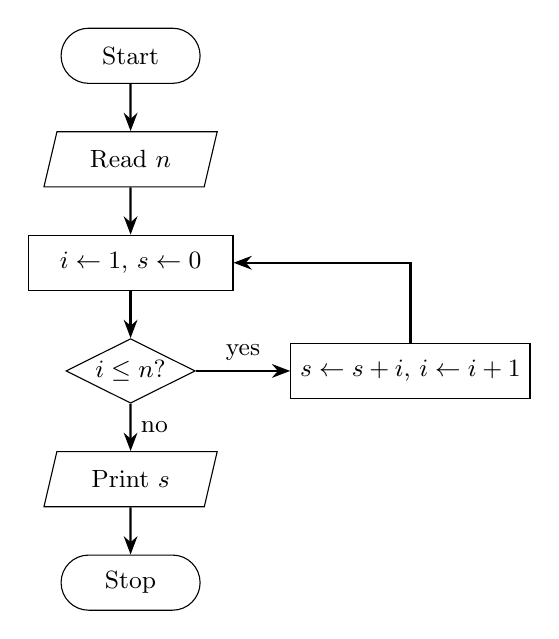
\begin{tikzpicture}[
  node distance=6mm and 12mm,
  every node/.style={font=\small},
  terminal/.style={rounded rectangle, draw, minimum width=20mm, minimum height=7mm},
  process/.style={rectangle, draw, minimum width=26mm, minimum height=7mm},
  io/.style={trapezium, trapezium stretches body, trapezium left angle=70, trapezium right angle=110, draw, minimum width=22mm, minimum height=7mm},
  decision/.style={diamond, aspect=2, draw, inner sep=1pt},
  arrow/.style={-{Stealth}, thick},
]
  \node[terminal] (start) {Start};
  \node[io, below=of start] (read) {Read $n$};
  \node[process, below=of read] (init) {$i \gets 1$, $s \gets 0$};
  \node[decision, below=of init] (test) {$i \le n$?};
  \node[process, right=of test] (add) {$s \gets s + i$, $i \gets i + 1$};
  \node[io, below=of test] (print) {Print $s$};
  \node[terminal, below=of print] (stop) {Stop};

  \draw[arrow] (start) -- (read);
  \draw[arrow] (read) -- (init);
  \draw[arrow] (init) -- (test);
  \draw[arrow] (test) -- node[above] {yes} (add);
  \draw[arrow] (add) |- (init);
  \draw[arrow] (test) -- node[right] {no} (print);
  \draw[arrow] (print) -- (stop);
\end{tikzpicture}
